% This is samplepaper.tex, a sample chapter demonstrating the
% LLNCS macro package for Springer Computer Science proceedings;
% Version 2.20 of 2017/10/04
%
\documentclass[11pt]{llncs}

%
\usepackage[bindingoffset=0mm,margin=2.5cm]{geometry}
\usepackage{graphicx}
\usepackage{float}
\usepackage[ ]{algorithm2e}
\usepackage{newtxmath}
\usepackage{fixltx2e}
\usepackage[printonlyused,withpage]{acronym}
\usepackage{hyperref}


\def\SPSB#1#2{\rlap{\textsuperscript{#1}}\textsubscript{#2}}


% Used for displaying a sample figure. If possible, figure files should
% be included in EPS format.
%
% If you use the hyperref package, please uncomment the following line
% to display URLs in blue roman font according to Springer's eBook style:
% \renewcommand\UrlFont{\color{blue}\rmfamily}

\begin{document}
%
\title{Analzying Different Approaches for finding Vertex-Cover\\ ECE 650 - Project Report\thanks{Supported by University of Waterloo}}
%
%\titlerunning{Abbreviated paper title}
% If the paper title is too long for the running head, you can set
% an abbreviated paper title here
%
\author{Uditya Laad\orcidID{20986041} (\email{ulaad@uwaterloo.ca})
\\ Swapnil Baluja\orcidID{20933848} (\email{s3baluja@uwaterloo.ca})}
% Third Author\inst{3}\orcidID{2222--3333-4444-5555}}
%
\authorrunning{Authors: Uditya Laad, Swapnil Baluja}
% First names are abbreviated in the running head.
% If there are more than two authors, 'et al.' is used.
%
\institute{University of Waterloo, Waterloo, ON, N2L 3G1, CA\\
%\url{url}
}

%
\maketitle              % typeset the header of the contribution
%

\vspace{-6mm}


\begin{abstract}
	We are comparing the time and output effieciency of different algorithms used for finding Minimum Vertex-Cover of a Graph. The algorithms being considered are CNF-SAT-VC, APPROX-VC-1, and APPROX-VC-2.

	\keywords{Running Time  \and Approximation Ratio \and Number of Vertices}
\end{abstract}

\vspace{-17mm}
	
$\>$ $\>$ $\>$ 
	\begin{table}[!]	
		\centering
		\setlength{\tabcolsep}{6pt}
		\begin{tabular}{l l l}
			\textbf{Abbreviations:} & n & Number of Vertices\\
			& k & Size of Proposed Vertex Cover\\
			& E & Edges of Graph\\
			& Std. Dev. & Standard Deviation\\
			& VC-1 & APPROX-VC-1\\
			& VC-2 & APPROX-VC-2\\
			& CNF & Conjunctive Normal Form\\
			& SAT & Satisfiable
		\end{tabular}
	\end{table}

%	\begin{acronym}
%		\acro {n} {Number of Vertices}
%		\acro {k} {Size of Proposed Vertex Cover}
%		\acro {Std. Dev.} {Standard Deviation}
%	\end{acronym}



%
%
%

\vspace{-10mm}
\section{Algorithms Being Considered}
\subsection{CNF-SAT-VC}
	\begin{algorithm}[H]
		\caption{CNF-SAT-VC}\label{getgpx}

		\DontPrintSemicolon
		\SetAlgoLined

		\KwIn{G=(n,E): Graph with $n$ number of Vertices and $E$ Edges}
		\KwOut{VertexCover[]}\;

		Initialize k = 1\;
		\While{k $\leq$ v}{
			minisat\_CNF =  createClausesForVertexCoverProblem()

			SATISFIABILITY, vertexCover = Minisat.Solve(minisat\_CNF)

			\;

			\If {SATISFIABILITY == true} {
				return vertexCover
			}\;

			k++
		}
	\end{algorithm}

	.\\
	This algorithm makes use of Minisat Solver \cite{minisat} to find the optimal Vertex-Cover (i.e. the Minimum possible Vertex-Cover, required to cover all edges)\\\\


\subsection{APPROX-VC-1}
	\vspace{-1mm}
	
	\begin{algorithm}[H]
		\caption{APPROX-VC-1 \cite{prj_pdf}}\label{getgpx}

		\DontPrintSemicolon
		\SetAlgoLined

		1. \textbf{Set:} v\_high = Vertex with highest degree (most incident edges).\;
		2. Add 'v\_high' to VertexCover[]\;
		3. Throw away all edges incident to 'v\_high'.\;
		4. Repeat $'Steps \,\, 1-3'$ till no edges remain.\;
	\end{algorithm}


\subsection{APPROX-VC-2}
	\vspace{-2mm}

	\begin{algorithm}[H]
		\caption{APPROX-VC-2 \cite{prj_pdf}}\label{getgpx}

		\DontPrintSemicolon
		\SetAlgoLined


		1. \textbf{Set:} first\_edge =  First available 'Edge(src,dest)' in the Graph\;
		2. Add both 'src' and 'dest' to VertexCover[]\;
		3. Throw away all edges attached to 'src' and 'dest'.\;
		4. Repeat $'Steps \,\, 1-3'$ till no edges remain.\;
	\end{algorithm}




\section{Analyzing with Original Encoding\cite{a4_pdf}}
    \subsection{Running-Time}

	\noindent We compute the Mean and Standard Deviation of CPU-Time taken by each algorithm for multiple graph inputs, grouped over 'No. of Vertices (v)'.

	\subsubsection{CNF-SAT-VC}.\\
		
		From Fig. \ref{fig1}, we can make out that 'CNF-SAT-VC' takes the longest to find the Vertex Cover.
		It competes well with the other 2 algorithms till $n \leq 10$, as compromising on a few milliseconds is no big deal, especially when we take the optimal vertex-cover into consideration.
		
		But for $n \geq 10$, the running-time drastically shoots up. This is because, with increasing number of Verticies, we also have more and more edges to cover; leading to a higher value of 'k' to find an optimal solution. This increases the number of clauses that are being input to the Minisat-Solver to determine satisfiability. Also, the clauses being added are not definite, but rather complex.

		The total number of clauses required for each value of 'k' is given by the following equation: \cite{a4_pdf}
		\begin{equation}
			Number \, of \, Clauses = k + n(\SPSB{k}{2}) + k(\SPSB{n}{2}) + |E|
		\end{equation}

		Where: 'k' is the size of proposed Vertex-Cover, 
			  'n' is the Number of Vertices, 
			  and 'E' contains all the edges in the Graph

		This leads to a CNF with a lot of complex clauses, that require more resources and time to be solved by Minisat. (Note: that this is an NP-Complete problem; i.e: it cannot be solved in poynomial time.)

		Also, we start with k=1, and keep using the minisat solver until we get a satifiable result. Hence, even for a slight increase in satifiable 'k', the required CPU-time shoots up by a huge margin; as we are solving '$\forall$ k $\in$ [1, Satisfiable\_k]'.

		However, we notice that for n $\geq$ 20, the running time is exactly 10 seconds, which contradicts the above reasoning. This constant run-time is the result of 'timeouts'.
		For large enough 'n', it is possible that 'CNF-SAT-VC' may take a very long time (could be hours or days or even weeks), which is obviously not feasible. Hence, we timeout the algorithm once a specified amount of CPU-time has been utilised for any run.\\

		\begin{figure}[H]
			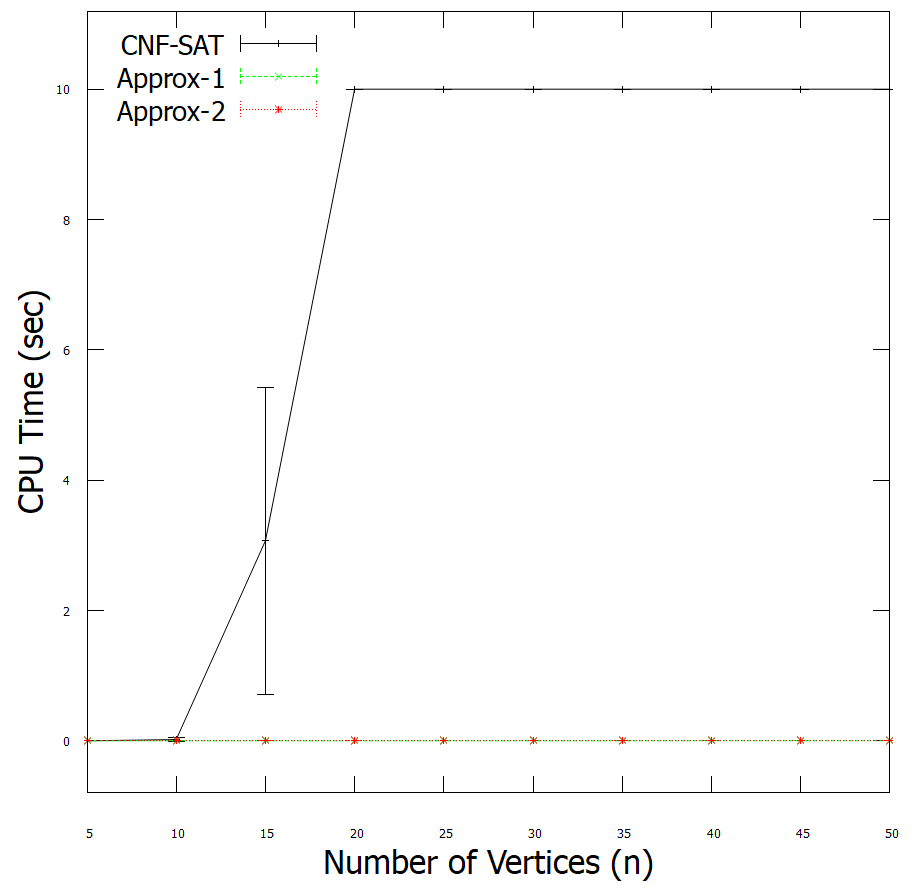
\includegraphics[width=0.84\textwidth]{original_time_vs_n.png}
			\caption{Graph of 'Running (CPU) Time (sec)' v/s 'Number of Vertices (n)', for each algorithm being considered and using Original Encoding \cite{a4_pdf} in CNF-SAT-VC} \label{fig1}
		\end{figure}

		\vspace{-7mm}
		
		Standard Deviation, which is represented by a vertical bar at each marked coordinate in Fig. \ref{fig1},  shows the amount by which the running-time of each input at 'n' differs from the mean running-time at that 'n'.
		\vspace{-2mm}
		\begin{itemize}
  			\item At n$\geq$ 20, we see that the standard deviation is Zero. This is because 'CNF-SAT-VC' times out for each input provided at n$\geq$20. And since the timeout value is considered when performing analysis, there is no difference between the running times of each input; resulting in no standard deviation between those runs.
 			\item Table-1 shows the values we've plotted on the graph (Fig. \ref{fig1}) for 'CNF-SAT-VC'. When compared against their respective mean values, we will observe that the standard deviations are quite large. This is because we have good variations in our input graphs. This also means that the time taken by CNF-SAT-VC depends heavily on the complexity of Graph input and that of the clauses derived from it.
		\end{itemize}
		
		\vspace{-8mm}

		\begin{table}
			\caption{Mean and Standard Deviation in CPU Time - for CNF-SAT-VC}\label{tab1}
			\setlength{\tabcolsep}{12pt}
			\begin{tabular}{| l | l | l | l | l |}
				\hline
				No. of Vertices & 5 & 10 & 15 & 20 \\
				\hline
				Mean (CPU Time) & 0.000202  & 0.018633 & 3.066866 & 10.000000 \\
				Standard Deviation & 0.000074  & 0.030873 & 2.354415 & 0.000000 \\
				\hline
			\end{tabular}
		\end{table}
    	
	\vspace{-5mm}
    
	\subsubsection{APPROX-VC-1 and APPROX-VC-2}.

		By looking at the graph (in Fig. \ref{fig1}), it appears as if APPROX-VC-1 and APPROX-VC-2 take the same amount of CPU-time to find the vertex cover. Some may even say they both take 0 seconds to produce the output. But, this is not true. The time taken by either algorithm does not exceed 1 millisecond for the tested data. And since our scale for 'Running Time' is in seconds, the graph gives an impression that they both take the same time. This is expected, since both these algorithms run in polynomial time, unlike 'CNF-SAT-VC' which was previously discussed.\\

		Table-2 shows the values we've plotted for these two algorithms in Fig. \ref{fig1}. On comparing their mean CPU-time at each 'n', we can make out that the time taken by APPROX-VC-2 is about 45-55\% less than that of APPROX-VC-1. The difference could possibly be a result of the overhead involved in finding the Vertex with highest degree for each iteration in APPROX-VC-1, which leads to more CPU-time; compared to APPROX-VC-2 which simply picks the first available edge in the list.

		\vspace{-8mm}

		\begin{table}
			\caption{Mean and Standard Deviation in Time - APPROX-VC-1 \& APPROX-VC-2}\label{tab1}
			\begin{tabular}{|l|l|l|l|l|l|l|l|l|l|l|l|}
				\hline
				No. of Vertices &  & 5 & 10 & 15 & 20 & 25 & 30 & 35 & 40 & 45 & 50 \\

				\hline
				APPROX-VC-1 & Mean & 0.000019 & 0.000042 & 0.000079 & 0.000139 & 0.000203 & 0.000273 & 0.000351 & 0.000469 & 0.000569 & 0.000686 \\
				& Std. Dev.& 0.000005 & 0.000003 & 0.000006 & 0.000006 & 0.000014 & 0.000014 & 0.000018 & 0.000019 & 0.000029 & 0.000033 \\
				\hline
				APPROX-VC-2 & Mean & 0.000013 & 0.000025 & 0.000041 & 0.000067 & 0.000096 & 0.000128 & 0.000155 & 0.000204 & 0.000245 & 0.000282 \\
				& Std. Dev. & 0.000001 & 0.000002 & 0.000004 & 0.000006 & 0.000008 & 0.000010 & 0.000013 & 0.000009 & 0.000018 & 0.000017 \\
				\hline
			\end{tabular}
		\end{table}
		
		\vspace{-5mm}
		
		A realtively smaller Standard Deviation at each 'n', also means that the Mean values are good enough to draw concrete conclusions with respect to CPU-time taken by APPROX-VC-1 and APPROX-VC-2.
		
		
	\subsubsection{Overall}
		\vspace{-2mm}
		\begin{itemize}
			\item On the basis of above analysis, we belive it's safe to say that APPROX-VC-2 is the fastest of all the three algorithms being considered, with APPROX-VC-1 being the next best.
			\item CNF-SAT-VC still performs reasonably fast for n $\leq$ 10, although still not as fast as the other two. But falls behind for further values of 'n' and that too by a huge margin.
			\item This is not surprising, as CNF-SAT-VC is NP-Complete, whereas the other 2 algorithms run in polynomial time.
		\end{itemize}

    \subsection{Approximation Ratio}
	\vspace{-9mm}

	\begin{figure}[H]
		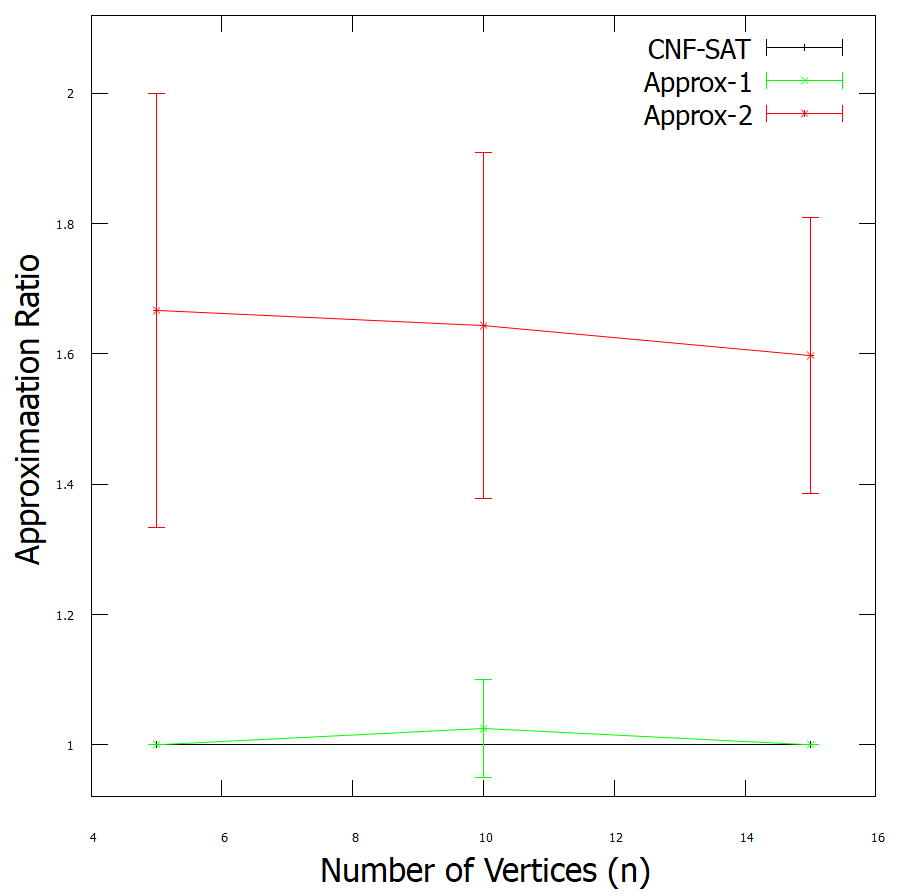
\includegraphics[width=0.4\textwidth]{original_ar_vs_n.png}
		\caption{Graph of 'Approximation Ratio' v/s 'Number of Vertices (n)', using Original Encoding \cite{a4_pdf} in CNF-SAT-VC} \label{fig2}
	\end{figure}

	\vspace{-6mm}

	This will be explained in Section 3.2, since we have a larger set of data in the graph (to compare against) with the Optimized version of CNF-SAT-VC.\\

\section{Optimizing CNF-SAT-VC}
	\textbf{Note:} Pendant Edge refers to an edge, whose either or both end-point(s) is a  pendant-vertex (Vertex with only one incident edge).\\

	The above analysis (in Section 2) was performed for the Encoding that had been provided by Professor Arie in Assignment\_4.pdf \cite{a4_pdf}. The original encoding can be improved by revising it.\\
%	1] Vertices with zero incident edges should never be included in the vertex-cover.
%		\begin{equation}
%			 \forall \, i \in \{[1, n]:  i \,\, has \,\, no \,\, incident \, edge\}; \,\,\, \forall j \in [1, k]:\,\,
%			Definite \,\, clause  \,\, (\neg x\textsubscript{i,j})
%		\end{equation}

%	\noindent 2] For a pendant edge, the pendant vertex or any one vertex (in case both are pendant) should not be included in the vertex cover. 
%		\begin{equation}
%			 \forall \, (i,j) \in \{E:  i \,\, and/or \,\, j \,\, has \,\, exactly \,\, one \,\, incident \, edge\}; \,\,\, \forall j \in [1, k]:\,\,
%			Definite \,\, clause  \,\, (\neg x\textsubscript{m,j})
%		\end{equation}
%		$\>$ $\>$ $\>$  \textbf{where:} m = Vertex with minimum no. of incident edges (among 'i' and 'j').\\
	
%	\noindent The above 2 conditions will add definite clauses with exactly one atom. This will help Minisat-Solver solve the problem faster, as it will already know the assignment of atomic propositions added using these clauses as 'False'.\\

%	\noindent Another alternative is, instead of adding the negation of these atomic propositions as clauses, simply do not have these atomic propositions, and also revise the original reduction \cite{a4_pdf} to exclude them from clauses.\\

	\begin{algorithm}[H]
		\caption{Finding Redundant and Mandatory End-points in Pendant Edges}\label{algorithm4}

		\DontPrintSemicolon
		\SetAlgoLined

		\KwIn{G=(n,E): Graph with 'n' number of Vertices and 'E' Edges}
		\KwOut{redundantVertices[]: Vertices that are not required in minimum vertex-cover.\\
			$\>$ $\>$ $\>$ $\>$ $\>$ $\>$ $\>$ $\>$ mandatoryVertices[]: (Unique) Set of vertices that must be a part of the minimum vertex-cover.}\;
		
		Initialize x = 0\;
		\While{$x < |E|$}{
			\If {E[x] is a Pendant Edge} {
				\If {$|Incident\_edges \,\, of \,\, E[x].src| == 1$} {
					redundantVertices.add(E[x].src)\;
					mandatoryVertices.add(E[x].dest)
				}
				\Else {
					redundantVertices.add(E[x].dest)\;
					mandatoryVertices.add(E[x].src)
				}
			}\;

			\vspace{-3mm}

			x++
		}\;
		
		\vspace{-3mm}

		mandatoryVertices.removeDuplicates();
		\;.
	\end{algorithm}

	.\\

	\noindent \textbf{The revised reduction will be as follows:} \cite{a4_pdf}\\
	Given a pair $(G, k)$, where $G = (V,E)$, denote $|V| = n$. Assume that the vertices are named $1, . . . , n$. Construct $F$ as follows.
	
	\vspace{-5mm}

	\begin{gather*}
		Let \,\, A \,\, =  \,\, Set \,\, of \,\, Mandatory-Verticies \,\,  (which \,\, must \,\, be\,\, a \,\, part \,\, of \,\, Minimum \,\, Vertex-Cover)\\
		Let \,\, B \,\, =  \,\, Set \,\, of \,\, redundant \,\, vertices, \,\,  (which \,\, are \,\, not \,\, required\,\, to \,\, be \,\, a \,\, part \,\, of \,\, Minimum \,\, Vertex-Cover)\\
		(Both \,\, 'A' \,\, and \,\, 'B' \,\, are \,\, found \,\, using \,\, Algorithm-\ref{algorithm4})
	\end{gather*}

	\vspace{-8mm}

	\begin{gather*}
		Let \,\, N \,\, =  Set \,\, of  \,\, Vertices \,\, with \,\, no \,\, incident \,\, edges \,\, at \,\, all\\ \\
	\end{gather*}

	\vspace{-20mm}
	
	\begin{gather*}
		Let \,\, 'R' \,\, be \,\, a \,\, set \,\, of \,\, verticies \,\,  i  \in \{[1, n]: such \,\, that \,\,  i \,\, has \,\, no \,\, incident \, edge,\\
		or\,\,  i \,\, is \,\, a \,\, redundant \,\, endpoint \,\, in \,\, a \,\, pendant \,\, edge \};\\
		i.e. \,\,\,\, R \,\, = \{N \,\, \cup \,\, B\}
	\end{gather*}

	\noindent \textbf{NOTE:} 'Eligible Vertices' are vertices that do not belong to $\{A \,\, \cup \,\, R\}$; and 'Remaining Spaces' refer to the spaces remaining in vertex-cover after adding all elements of 'Set A'.\\

	The reduction uses '$(n - |R|) \, x \, k$' atomic propositions, denoted  $x\textsubscript{i,j}$, where $i \in \{[1, n] - R\}$ and $j \in [1, k]$. A vertex cover of size $k$ is a list of $k$ vertices. An atomic proposition $x\textsubscript{i,j}$ is true if and only if the vertex $i$ of $V$ is the $jth$ vertex in that list.\\
	
	\begin{algorithm}[H]
		\caption{CNF-SAT-VC - Revised Encoding}\label{algorithm5}

		\DontPrintSemicolon
		\SetAlgoLined

		\If {$k < |A|$} {
			Cannot have a vertex-cover of size 'k' for Graph 'G', i.e. (G,k) is unsatisfiable.
		}
		\Else {
			Use the following set of clauses to determine satisfiability:

	\noindent 1] All Mandatory Vertices (in Set A) must be included in the Vertex Cover.
			\vspace{-2mm}
			\begin{gather*}
				\,\, \forall i \in [1,|A|]:\,\,\,  a \,\, clause  \, (x\textsubscript{A[i],i});\\
				and\,\, \forall i \in [1,|A|], \,\, \forall j \in \{[1,n], \,\, j\neq A[i]\}:\,\,\,  a \,\, clause  \, (\neg x\textsubscript{j,i})\\
				and\,\, \forall i \in [1,|A|], \,\, \forall j \in \{[1,k], \,\, j\neq i\}:\,\,\,  a \,\, clause  \, (\neg x\textsubscript{A[i],j})
			\end{gather*}

	\noindent 2] At least one eligible vertex is the ith vertex in the remaining spaces of Vertex Cover.
			\vspace{-2mm}
			\begin{gather*}
				\forall j \in [|A| + 1, k]:\,\,\,  a \,\, clause  \, (x\textsubscript{i1,j} \, \lor \, x\textsubscript{i2,j} \, \lor \, ...... )\\
				where: \,\, \{i1,i2, .....\} = \{[1,n] - R - A\}
			\end{gather*}

	
	\noindent 3] No one (eligible) vertex can appear twice in the remaining spaces of Vertex Cover.
		\vspace{-2mm}
			\begin{gather*}
				\forall \,m \in \{[1, n] - R - A\}, \,\, \forall p,q \in [|A| + 1, k]\,\,\,  with \,\, p < q \,\, : \,\, a \,\, clause  \, (\neg x\textsubscript{m,p} \, \lor \, \neg x\textsubscript{m,q})
			\end{gather*}
	
	\noindent 4] No more than one eligible vertex appears in the mth position of the remaining spaces of Vertex Cover.
		\vspace{-2mm}
			\begin{gather*}
				\forall \, m \in [|A| + 1, k], \,\, \forall p,q \in \{[1, n]-R-A\} \,\, with \,\, p < q, \,\,
				 : \,\, a \,\, clause  \, (\neg x\textsubscript{p,m} \, \lor \, \neg x\textsubscript{q,m})
			\end{gather*}

	
	\noindent 5] Every \textbf{Uncovered-Edge} is incident to at least one vertex in the vertex cover.
		\vspace{-2mm}
			\begin{gather*}
				\forall \, (i,j) \in E, such \,\, that: i \notin A \,\, and \,\,  j \notin A: \\
				a \,\, clause  \,\, (x\textsubscript{i,$|A|$+1} \, \lor \, x\textsubscript{i,$|A|$+2} \, \lor \, ....  \lor \, x\textsubscript{i,k} \lor \, \, x\textsubscript{j,$|A|$+1} \, \lor \, x\textsubscript{j,$|A|$+2} \, \lor \, ....  \lor \, x\textsubscript{j,k}\,)
			\end{gather*}


			}
		\end{algorithm}
	
	\vspace{4mm}

	The condition $k < |A|$ in Algorithm \ref{algorithm5} helps to skip running the minisat-solver for some UNSATISFIABLE values of 'k' (in certain cases), which help save time, specific to those cases.\\

	The revised encoding uses less atomic propositions, compared to the original one. Also we have a lot of definite clauses (with one atomic proposition). This helps simplify the CNF, which then helps Minisat solve it faster.

\newpage
     \subsection{Running Time}
	\vspace{-8mm}

	\begin{figure}[H]
		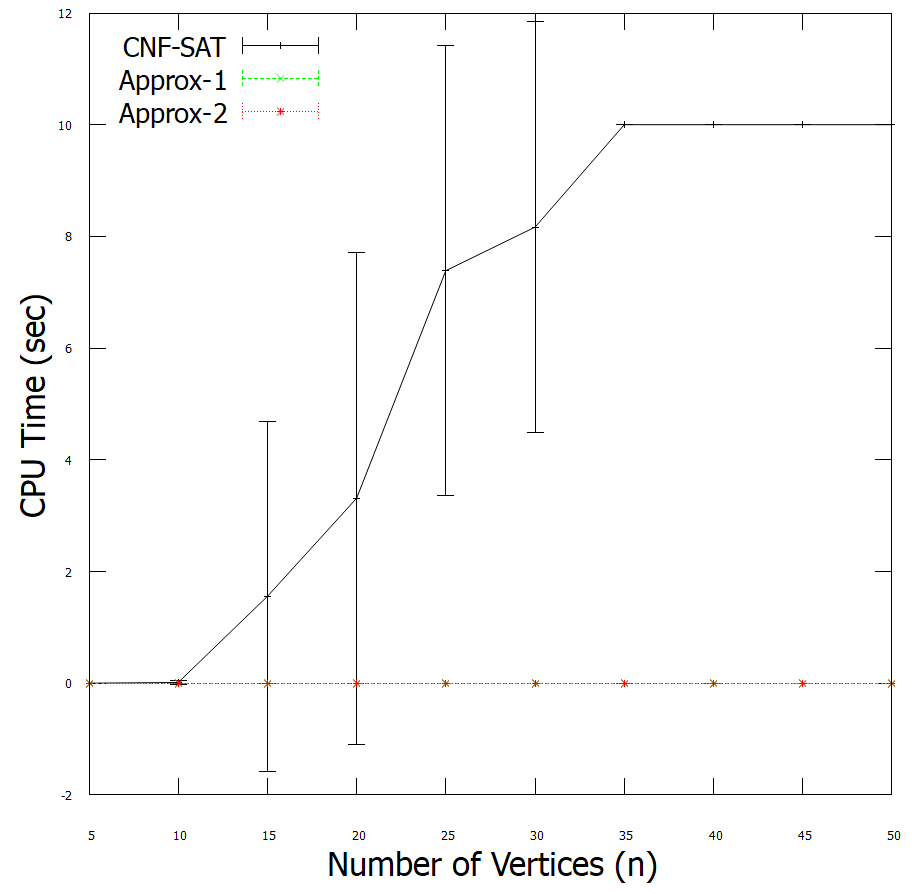
\includegraphics[width=0.88\textwidth]{optimized_time_vs_n.png}
		\caption{Graph of 'Running (CPU) Time (sec)' v/s 'Number of Vertices (n)', for each algorithm being considered and using Optimized Encoding in CNF-SAT-VC} \label{fig3}
	\end{figure}
	
	\vspace{-6mm}

	On comparing Figure \ref{fig1} with Figure \ref{fig3}, it's quite evident that the Optimized Encoding does scale to larger instances. The original encoding could not produce any output for graphs with $n \ge 20$, when timeout was kept to 10 sec. But the limit is now raised to 'n = 35', for the same time-out.

	As expected, we see that the CPU Time shoots up, for graphs with $n > 10$. But the rise is steeper, when compared with the original encoding. At v=15, we get no timeouts; hence the only reason for the large standard deviation can be attributed to good amount of variations in the input data. For $n \ge 25$, the optimized version does timeout for a lot of runs; and hence the large standard deviation.

	For $n \ge 35$, the optimized version times out for all runs, hence we see a consistent CPU time of 10 seconds (which is the timeout itself), with no standard deviation at all.

	Due to the large sample size of test data, it was not practical to try this analysis with a large value of timeout. But we did try executing certain input graphs with $n \ge 20$ (using the original encoding) one by one, and none of them could produce an output within 30 mins. This gives us a good indication of how significant the improvement (in Optimized Encoding) is.
 
\newpage
     \subsection{Approximation Ratio}
		\begin{figure}[H]
			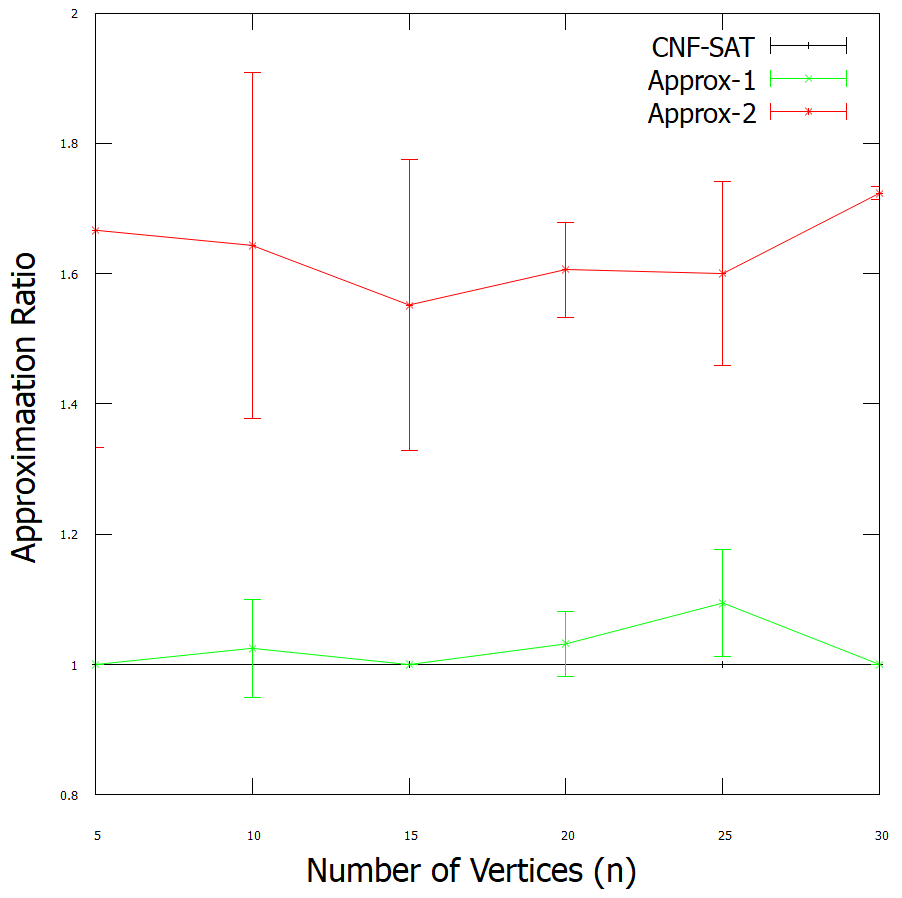
\includegraphics[width=0.75\textwidth]{optimized_ar_vs_n.png}
			\caption{Graph of 'Approximation Ratio' v/s 'Number of Vertices (n)', for each algorithm being considered and using Optimized Encoding in CNF-SAT-VC} \label{fig4}
		\end{figure}


		Approximation Ratio is computed using the following formula: \cite{prj_pdf}
	\begin{equation}
		ApproximationRatio(Algo) = \frac {|\,VertexCover(Algo)\,|} {|\,OptimalVertexCover\,|}
	\end{equation}
	
	Where: 'Algo' is the current algorithm being considered, 
		  'VertexCover(Algo)' is the Vertex-Cover found using 'Algo'
		  and 'OptimalVertexCover'  is the Minimum possible Vertex Cover.


	\subsubsection{CNF-SAT-VC}.\\

		CNF-SAT-VC always produces the Minimum (Optimal) Vertex Cover, since it starts looking for a satisfiable 'k' beginning k=1, and returns it once found. Hence, the approximation ratio for CNF-SAT-VC, by above definition, will always be equal to 1, as is evident from the graph.

		Due to this, the Standard Deviation, will always be Zero at each value of 'n'. This is proved by the absence of vertical bars at each coordinate (for CNF-SAT-VC)  in the graph (Fig. \ref{fig4}).\\

		Fig. \ref{fig4} shows data only till $n = 30$. This is because, it's not possible to find Approximation-Ratio for $n > 30$, since CNF-SAT-VC is the only source of finding an optimal vertex-cover, but it times out for larger instances.

		Also, note that the Mean Approximation Ratio that we see in the Graph are only for those inputs, that did not time-out. Those that time-out are not considered at all, which is also the reason for no data beyond  n=30 (where all runs time-out).

	
	\subsubsection{APPROX-VC-1 and APPROX-VC-2}.\\
		
		APPROX-VC-1 performs better than APPROX-VC-2 due the difference in selection of vertices by respective algorithms.
		
		APPROX-VC-1 picks the highest-degree vertex in each iteration, covering maximum possible edges for that particular iteration \cite{prj_pdf}. There are chances that this may not give the most optimal solution, as it is always possible that the edges covered by the highest-degree vertex would have anyway been covered by other vertices, later added to the vertex-cover in subsequent iterations. Another case where it might fail to produce an optimal solution is when the algorithm leads to a combination of vertices, each of which covers at least one unique edge by itself, but still a different combination (with a smaller size) is sufficient to cover all edges. Yet, the number of redundant vertices (in Vertex-Cover) are highly unlikely to be greater than those produced by APPROX-VC-2.
		
		APPROX-VC-2 picks the first available uncovered edge and simply adds its 'source' and 'destination' to the vertex-cover. It is very much possible that one or both of these vertices do not have any other incident edge(s). In any case, this algorithm will surely end up adding atleast one redundant vertex (i.e. the end-point of last uncovered edge).And since it is possible for our input graphs to contain many such edges, this can add a lot of redundant vertices to the vertex-cover, depending on the selection of edges.\\

		The graph backs the above analysis. We see that APPROX-VC-1 performs better and even returns optimal solutions for all inputs at n=5 and n=10, as is evident by the absence of Standard Deviation at both the coordinates. A reasonable standard deviation at $n= \{15, 20, 25\}$ also means, there are chances that the algorithm could have produced an optimal solution for some graph inputs at these 'n'. Although we see an approximation ratio of '1' with no standard deviation at n=30, this need not necessarily be true if we had a larger timeout; as we are not considering timed-out  runs (in Optimized CNF-SAT-VC) as discussed earlier (and there are high chances that majority of runs at n=30 could have timed-out).\\

		APPROX-VC-2 on the other hand, is nowhere near to being optimal, as was expected. Also, the Standard Deviation is very large, which backs our claim of getting different number of redundant vertices (in vertex-cover), depending on the order of edges being selected.


	\subsubsection{Overall}.
		\begin{itemize}
			\item From the above analysis, it's obvious that CNF-SAT-VC  produces the most optimal solution.
			\item APPROX-VC-1 also performs reasonably well, even providing an optimal solution in a lot of cases. Overall, it is very close to optimal.
			\item APPROX-VC-2 is very unpredictable and will never produce an optimal solution. (Since it will have atleast one redundant vertex in the vertex-cover).\\
		\end{itemize}

\section{Conclusion}
	\begin{itemize}
		\item If time-efficiency is the only requirement, than APPROX-VC-2 comes across as the most suitable option.
		\item When output-efficiency (optimal result) is the only requirement, CNF-SAT-VC (with optimized encoding) is the best fit, as it is guaranteed to produce minimum vertex-cover.\\
		\item In cases, where both time-efficiency and optimality are important , we can explore the following options:

	  		1] Use optimized CNF-SAT-VC first. If it times out (adjust the timeout beforehand, as per requirement), then use APPROX-VC-1.\\
             		2] Use only APPROX-VC-1: Although it is not guaranteed to produce an optimal solution; it is safe to say that the solution will be very close to being optimal (on the basis of above analysis)\\
	\end{itemize}


%
% ---- Bibliography ----
%
% BibTeX users should specify bibliography style 'splncs04'.
% References will then be sorted and formatted in the correct style.
%
% \bibliographystyle{splncs04}
% \bibliography{mybibliography}
%
\begin{thebibliography}{9}
    \bibitem{a4_pdf}
    Author, Prof. Arie Gurfinkel.: uw-ece650-1221-a4.pdf (2022)
    
    \bibitem{prj_pdf}
    Author, Prof. Arie Gurfinkel.: uw-ece650-1221-prj.pdf (2022)
    
    \bibitem{graphGen}
    Owner, Prof. Arie Gurfinkel.: graphGen
    
    \bibitem{gnuPlot}
    GNU Plot Home Page, \url{http://gnuplot.sourceforge.net}.
    
    \bibitem{minisat}
    Minisat Home Page, \url{http://minisat.se/}.
\end{thebibliography}
\end{document}
